\documentclass[tikz,border=0pt]{standalone}
\usepackage[american]{circuitikz}
\usetikzlibrary{arrows.meta,calc,positioning,decorations.pathmorphing,patterns}
\definecolor{zyloTeal}{HTML}{174A5B}
\definecolor{zyloTealTwo}{HTML}{246B7A}
\definecolor{zyloInk}{HTML}{1F2933}
\definecolor{zyloSoft}{HTML}{EAF4F4}
\definecolor{zyloPaper}{HTML}{F8FAFB}
\definecolor{zyloLine}{HTML}{44606B}
\definecolor{zyloOrange}{HTML}{D97706}
\begin{document}
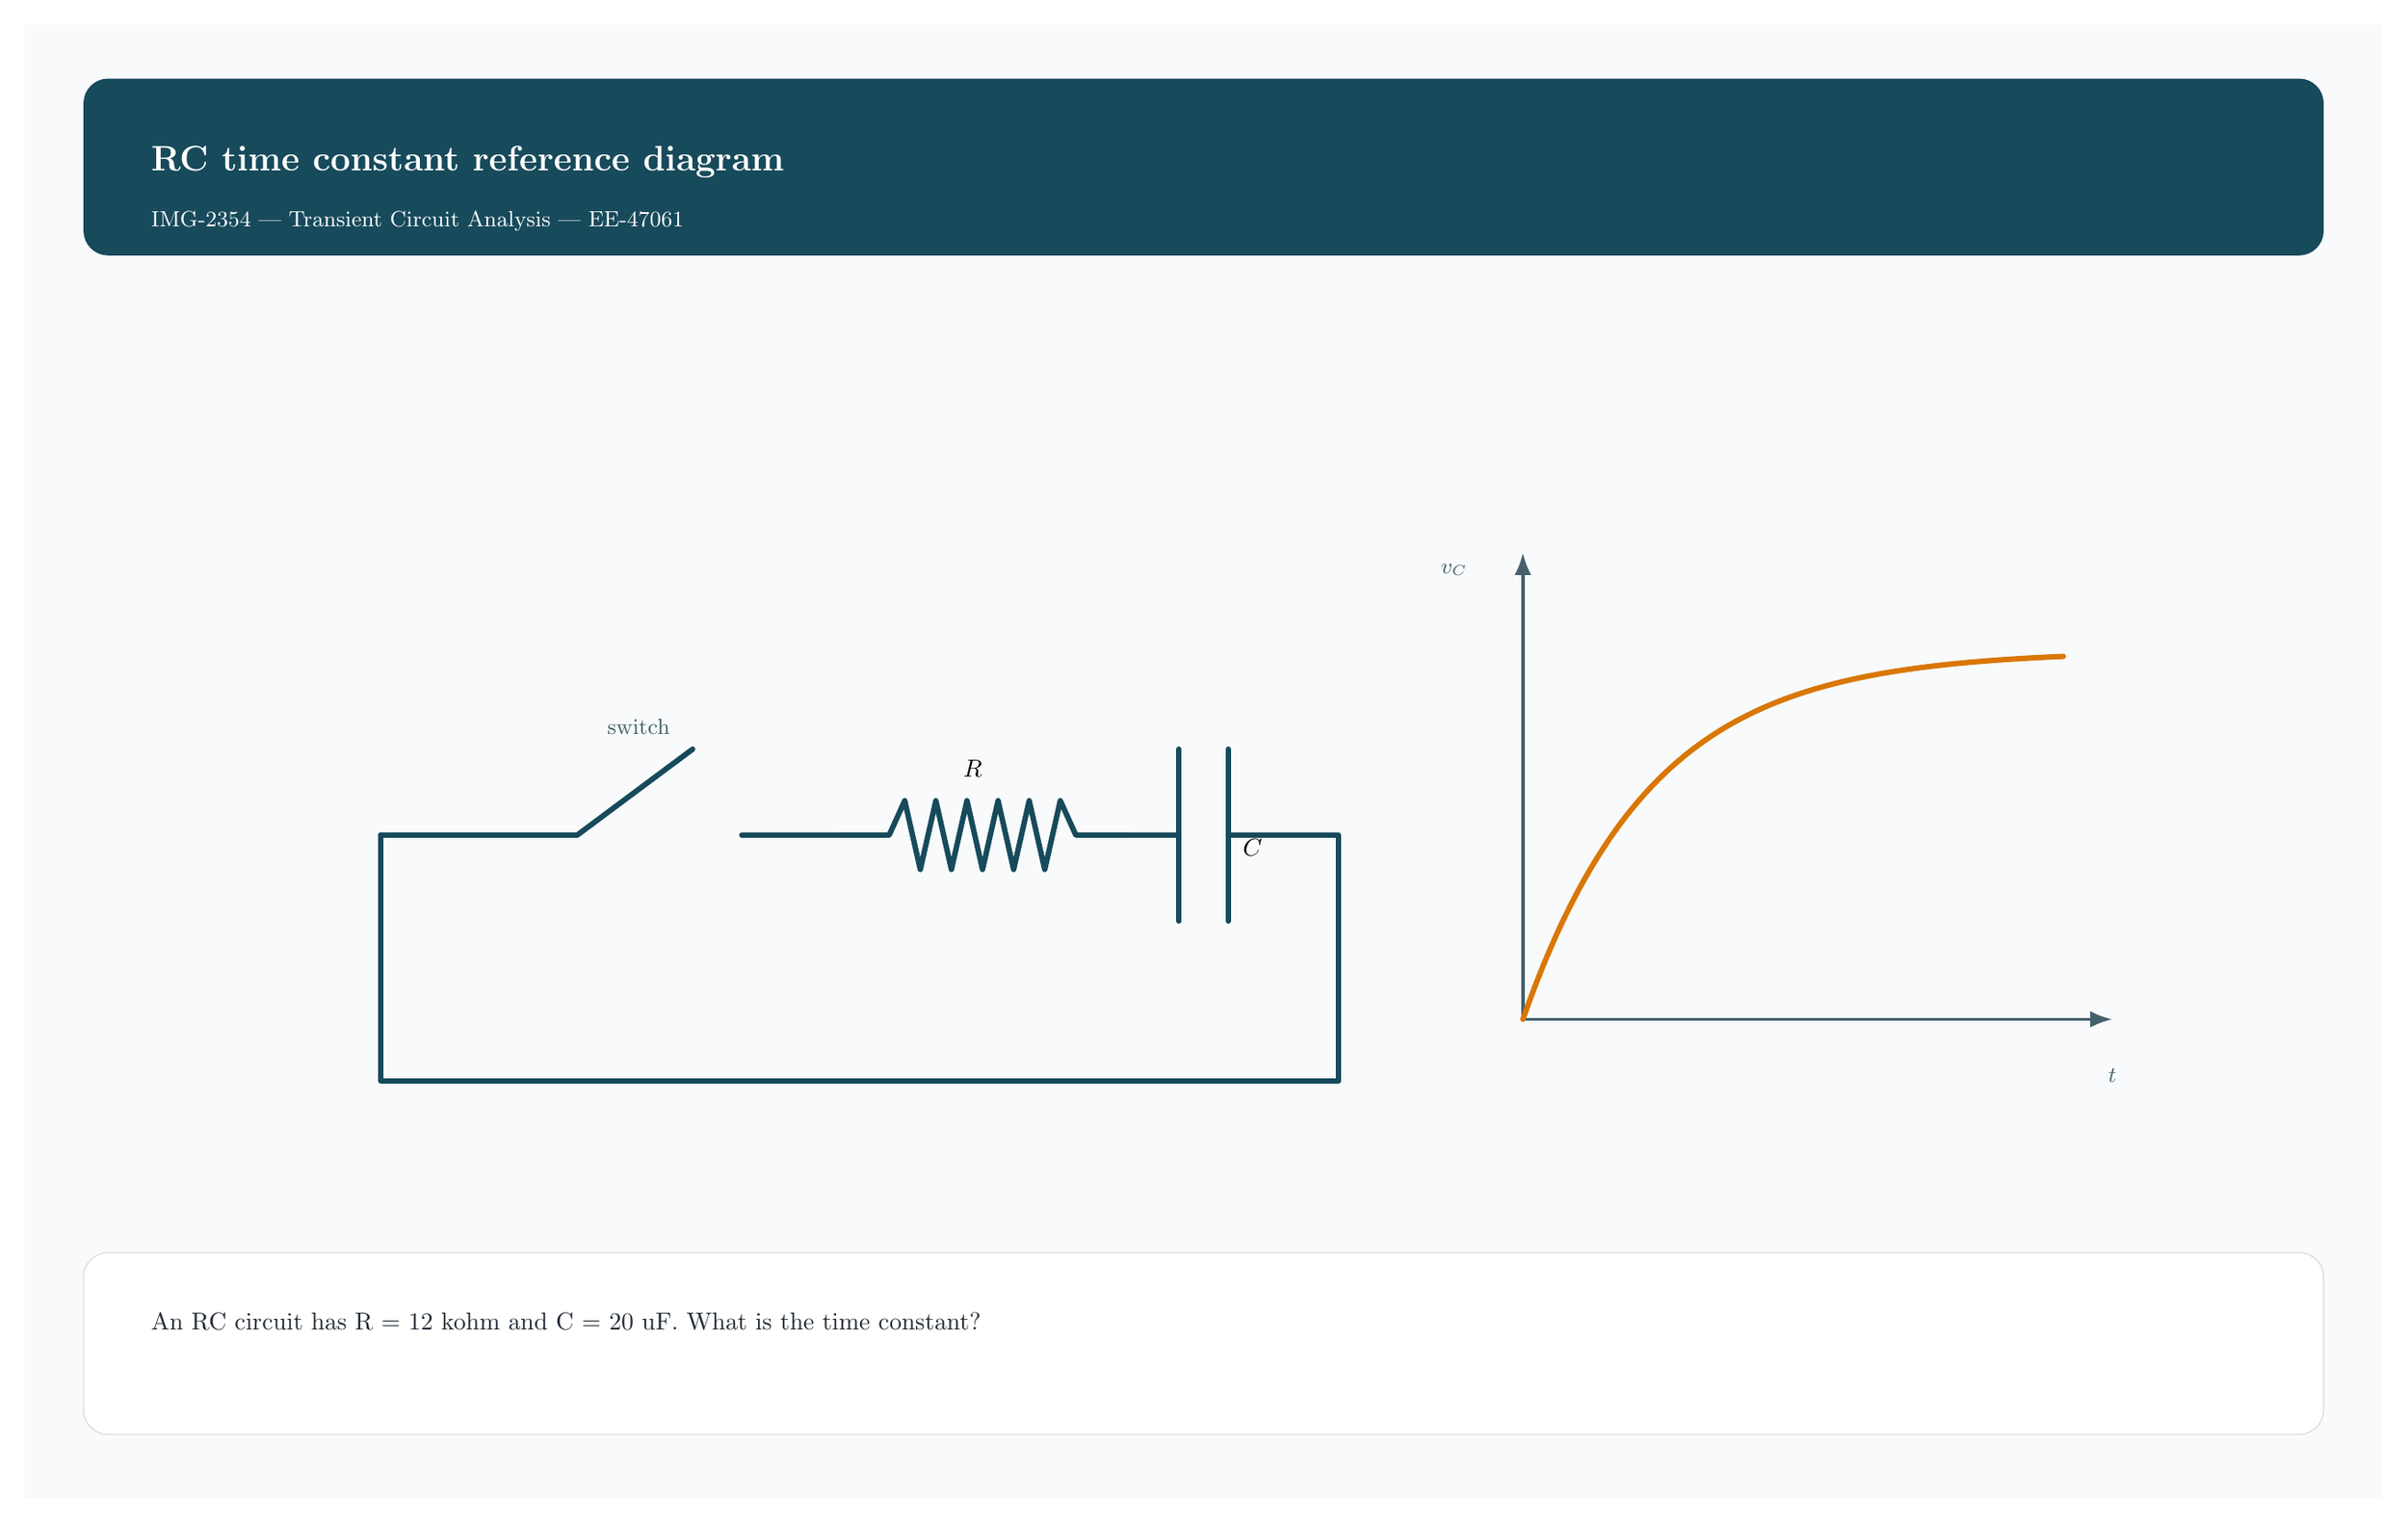
\begin{tikzpicture}[x=1pt,y=-1pt,>=Latex,line cap=round,line join=round]
\path[fill=zyloPaper] (0,0) rectangle (960,600);
\path[fill=zyloTeal,rounded corners=10pt] (24,22) rectangle (936,94);
\node[anchor=west,text=white,font=\bfseries\Large] at (48,56) {RC time constant reference diagram};
\node[anchor=west,text=white!82,font=\small] at (48,80) {IMG-2354 | Transient Circuit Analysis | EE-47061};
\tikzset{wire/.style={draw=zyloTeal,line width=2.2pt},thinwire/.style={draw=zyloLine,line width=1.35pt},accent/.style={draw=zyloOrange,line width=2.2pt},box/.style={draw=zyloTealTwo,fill=zyloSoft,line width=1.5pt,rounded corners=8pt}}
\draw[wire] (145,330) -- (225,330) -- (272,295);
\draw[wire] (292,330) -- (330,330);
\draw[wire] (330,330) -- (352,330) -- (352,330) -- (358.333,316) -- (364.667,344) -- (371,316) -- (377.333,344) -- (383.667,316) -- (390,344) -- (396.333,316) -- (402.667,344) -- (409,316) -- (415.333,344) -- (421.667,316) -- (428,330) -- (450,330);
\draw[wire] (450,330) -- (470,330);
\draw[wire] (470,295) -- (470,365); \draw[wire] (490,295) -- (490,365);
\draw[wire] (490,330) -- (535,330) -- (535,430) -- (145,430) -- (145,330);
\node[font=\small,text=zyloLine] at (250,286) {switch}; \node at (386,303) {$R$}; \node at (500,335) {$C$};
\draw[thinwire,->] (610,405) -- (850,405); \draw[thinwire,->] (610,405) -- (610,215);
\draw[accent] (610,405) -- (612.75,397.328) -- (615.5,390.049) -- (618.25,383.142) -- (621,376.588) -- (623.75,370.369) -- (626.5,364.468) -- (629.25,358.869) -- (632,353.557) -- (634.75,348.516) -- (637.5,343.733) -- (640.25,339.195) -- (643,334.889) -- (645.75,330.803) -- (648.5,326.926) -- (651.25,323.247) -- (654,319.757) -- (656.75,316.445) -- (659.5,313.302) -- (662.25,310.32) -- (665,307.491) -- (667.75,304.806) -- (670.5,302.259) -- (673.25,299.842) -- (676,297.548) -- (678.75,295.372) -- (681.5,293.307) -- (684.25,291.348) -- (687,289.489) -- (689.75,287.725) -- (692.5,286.051) -- (695.25,284.463) -- (698,282.956) -- (700.75,281.526) -- (703.5,280.17) -- (706.25,278.882) -- (709,277.661) -- (711.75,276.502) -- (714.5,275.402) -- (717.25,274.359) -- (720,273.368) -- (722.75,272.429) -- (725.5,271.538) -- (728.25,270.692) -- (731,269.889) -- (733.75,269.128) -- (736.5,268.405) -- (739.25,267.719) -- (742,267.069) -- (744.75,266.452) -- (747.5,265.866) -- (750.25,265.31) -- (753,264.783) -- (755.75,264.283) -- (758.5,263.808) -- (761.25,263.357) -- (764,262.93) -- (766.75,262.524) -- (769.5,262.139) -- (772.25,261.774) -- (775,261.428) -- (777.75,261.099) -- (780.5,260.787) -- (783.25,260.491) -- (786,260.21) -- (788.75,259.944) -- (791.5,259.691) -- (794.25,259.451) -- (797,259.223) -- (799.75,259.007) -- (802.5,258.802) -- (805.25,258.608) -- (808,258.423) -- (810.75,258.248) -- (813.5,258.082) -- (816.25,257.925) -- (819,257.775) -- (821.75,257.633) -- (824.5,257.498) -- (827.25,257.371) -- (830,257.249);
\node[font=\small,text=zyloLine] at (850,428) {$t$}; \node[font=\small,text=zyloLine] at (582,222) {$v_C$};
\path[draw=black!15,fill=white,rounded corners=10pt] (24,500) rectangle (936,574);
\node[anchor=west,text width=860pt,align=left,text=zyloInk,font=\normalsize] at (48,528) {An RC circuit has R = 12 kohm and C = 20 uF. What is the time constant?};
\end{tikzpicture}
\end{document}
